\documentclass[a4paper,ngerman,english]{amsbook} % Use book format.
\usepackage[T1]{fontenc}
\usepackage[utf8]{inputenc}
\usepackage{babel}

\usepackage{hyperref}
\usepackage{graphicx}
\usepackage{pifont}

\newcommand{\tick}{\ding{51}}
\newcommand{\fattick}{\ding{51}}

\frenchspacing


% ============================================================
% Markup macros for proof-reading
\usepackage{ifthen}
\usepackage[normalem]{ulem} % for \sout
\usepackage{xcolor}
\newcommand{\ra}{$\rightarrow$}
\newboolean{showedits}
\setboolean{showedits}{true} % toggle to show or hide edits
\ifthenelse{\boolean{showedits}}
{
	\newcommand{\ugh}[1]{\textcolor{red}{\uwave{#1}}} % please rephrase
	\newcommand{\ins}[1]{\textcolor{blue}{\uline{#1}}} % please insert
	\newcommand{\del}[1]{\textcolor{red}{\sout{#1}}} % please delete
	\newcommand{\chg}[2]{\textcolor{red}{\sout{#1}}{\ra}\textcolor{blue}{\uline{#2}}} % please change
}{
	\newcommand{\ugh}[1]{#1} % please rephrase
	\newcommand{\ins}[1]{#1} % please insert
	\newcommand{\del}[1]{} % please delete
	\newcommand{\chg}[2]{#2}
}
% ============================================================
% Put edit comments in a really ugly standout display
%\usepackage{ifthen}
\newboolean{showcomments}
\setboolean{showcomments}{false}
\newcommand{\id}[1]{$-$Id: scg-llncs.tex 30911 2010-02-05 10:21:47Z oscar $-$}
\newcommand{\yellowbox}[1]{\fcolorbox{gray}{yellow}{\bfseries\sffamily\scriptsize#1}}
\newcommand{\triangles}[1]{{\sf\small$\blacktriangleright$\textit{#1}$\blacktriangleleft$}}
\ifthenelse{\boolean{showcomments}}
{\newcommand{\nbc}[3]{
 {\colorbox{#3}{\bfseries\sffamily\scriptsize\textcolor{white}{#1}}}
 {\textcolor{#3}{\sf\small$\blacktriangleright$\textit{#2}$\blacktriangleleft$}}}
 \newcommand{\version}{\emph{\scriptsize\id}}}
{\newcommand{\nbc}[3]{\textcolor{#3}{#2}}
 \newcommand{\version}{}}
\newcommand{\nb}[2]{\nbc{#1}{#2}{orange}}
\newcommand{\here}{\yellowbox{$\Rightarrow$ CONTINUE HERE $\Leftarrow$}}
\newcommand\rev[2]{\nb{TODO (rev #1)}{#2}} % reviewer comments
\newcommand\fix[1]{\nb{FIX}{#1}}
\newcommand\todo[1]{\nb{TO DO}{#1}}
\newcommand\meta[1]{\nbc{META}{#1}{purple}}
\newcommand\jr[1]{\nbc{JR}{#1}{orange}}
\newcommand\nes[1]{\nbc{nes}{#1}{blue}}
\newcommand\on[1]{\nbc{ON}{#1}{teal}} % add more author macros here
\newcommand\ewe[1]{\nbc{EWE}{#1}{olive}} % add more author macros here


\title{DoodleDebug}

\begin{document}
\maketitle
\begin{figure}
	
\includegraphics[scale=0.25]{img/DoodleDebug-logo.png}
\end{figure}

\chapter*{Abstract}
Software developers actively make use of debugging tools in order to find problem sources in code. In relation to a previous paper\cite{dd-paper}, we designed and implemented a tool representing a new style of debugging: Objects are responsible of their own visual representation, as already seen in classical tools, but with a powerful and yet simple mechanism for graphical visualization rather than text only. Most of its power is gained when taking on conceptually multidimensional objects like lists of matrices.

\chapter*{Introduction}
\nes{Read and quote all publications assiciated with whyline: http://faculty.washington.edu/ajko/whyline-java.shtml}
\nes{Read: "http://www.amazon.com/Write-Point-Bill-Stott/dp/0231075499"}
\section*{Idea}
\meta{\\Fast start --> Ok like that?\\}
Debugging tools should save time. But when it comes to complex problems, like a list of matrices, classical tools like Java's \verb-System.out.println()- break down and become either expensive to use or completely useless\cite{dd-paper}. A Debugger may handle such problems better, it does not allow to compare two time slices. DoodleDebug combines graphical object representation with a simple API, still approving the simple and widely accepted usage pattern of \verb-System.out.println()-.
\meta{\\Main text\\}
For programmers, it's an everyday problem: Some feature of a program is not working correctly, but it's not clear where the problem originating from. The simplest approach, just staring at code and build some mental model to play the program in one's head, which is usually time and concentration intensive. In most cases, it's much more comfortable to automatically build a visual representation of runtime data, which is provided by debuggers for instance. They allow users to stop at a particular moment in time, the whole program state is inspectable and commonly used data types have some useful textual representation. One big problem here is that a program is only inspectable at one snapshot in time, but two states cannot directly be compared. Another widely used solution, printing on a console, eliminates this issue and has other advantages: Because such printing instructions are directly written into code to debug, which might be quicker or more convenient in some cases \todo{refer to study, where some subjects didn't use any debugger}. Also, printing to a console allows to precisely represent an object with needed data only using its \verb-toString()- method (in Java). \meta{Does this make sense now?} But still it lacks some features: On the one hand, the only supported output format is one-dimensional text, no colors, images or free spacial positioning. On the other hand, a line that has been printed cannot be edited any more, therefore advanced formatting becomes very complicated. \meta{Convinced about downsides?}
This paper introduces a solution which aims on eliminating the above mentioned disadvantages and includes a small qualitative study for its verification.

\nes{Please do read "write to the point", linked above. Among many other things, it explains quite nicely how to break text into paragraphs.}

\chapter*{Development}
\section*{Planning}

\subsection*{Sketching the Features}
The concept of a new system for code understanding, especially for multi-dimensional objects like matrices was already introduced and justified in a previous paper\cite{dd-paper}. One main result was that textual output is not powerful enough to produce useful output in some cases. Anther one was that customized representations of objects tend to have some common denominators, like including their class name. Base on this information, we started to sketch some candidate renderings and corresponding code snippets of commonly used data structures in pen and paper style, planning to throw away failures during the design process and focus only on good prototypes when going towards implementation. We tried to follow the principle of not mixing up the design and engineering  processes\cite{sketching-user-experiences}.

\subsection*{Confronting People With Hand Drawings}
After we had created a fair amount of sketches, we asked programmers to just have a look at our drawings and explain what they see (figure~\ref{sketch-discussion}). If they immediately anticipated the virtual situation, it was a good example and we kept it. If most candidates failed to understand what a particular drawing meant, or even took some wrong conclusions out of it, we either threw it away or tried to redesign, based on their statements and then re-evaluate with other people.

\begin{figure}[h]
	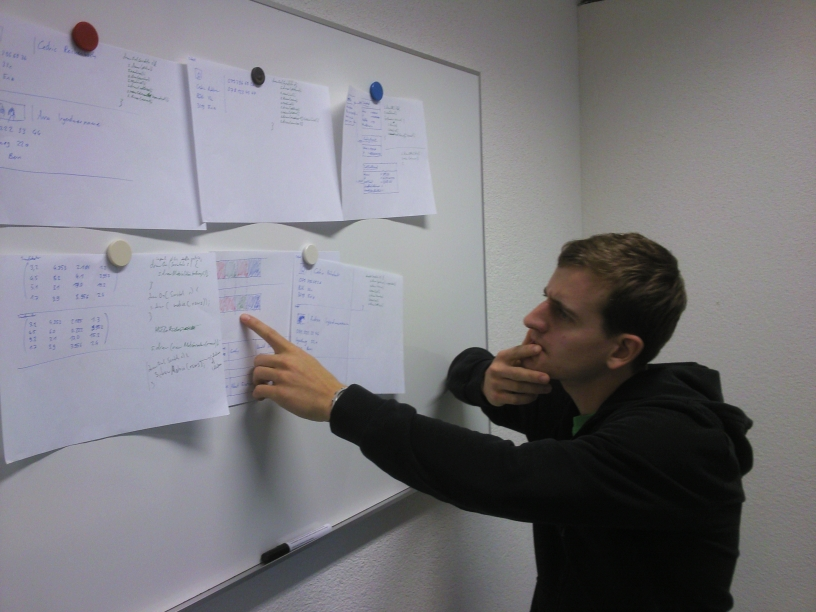
\includegraphics[width=\textwidth]{img/design-sketches_thinker.jpg}
	\caption[Confronting people with design sketches]{Programmers should look at our code snippets and corresponding design sketches for us to evaluate their intuitiveness}
	\label{sketch-discussion}
\end{figure}

\section*{Programming}
\nes{There should be text under every heading.}
\meta{What kind of text?}

\subsection*{Communication between Java Virtual Machines}
The calls for object visualizations are initiated directly from a user's program code, i.e. in the virtual machine (VM) where the user's program is running inside. DoodleDebug renders it's output into a view tab inside eclipse and must therefore be running in the same VM as eclipse. Since runtime information about objects and rendering calls must be provided from the user's VM to the eclipse VM, a solid communication mechanism is needed. After failing attempts with RMI, we switched SIMON (Simple Invocation of Methods Over Network)\cite{simon}, a simple alternative which allows to create a registry on a specified port of localhost and add a Server object to it. Clients can find the server through this registry and send messages to it by calling it's methods with simple objects like Strings as arguments.

\subsection*{Providing Code from Eclipse Plugin to Workspace}
\subsubsection*{Lack of Documentation} \meta{Probably throw this into appendix.}
In order to provide API functionality such as \verb-Doo.dle()- or the \verb-Doodleable- interface to users, we had to find some way of providing Java code automatically from our plugin to the current eclipse workspace. \nes{Don't talk about "had to find some way." In its way, this section has the least priority. It should probably be called "Implementation." Because it isn't very important, try and be brief: what were the implemtation challenges, what were the solutions? You're kind of saying that, just say it briefer.} One may say that everything is well-documented in the Eclipse documentation \nes{Too prosaic. Also: doesn't really matter. This is science.}, but the challenge was to find the right part in the documentation. Eclipse developer forums neither could help, but finally a hint was given by some Stackoverflow user: In order to provide code to workspace Java projects, a plugin needs to use the extension point \verb-org.eclipse.jdt.ui.classpathContainerPage-. From then on, another big help was the source code of JUnit, which uses the same technique, otherwise, it would probably have taken several more weeks until everything was working finely. \nes{Rewrite, away from what you did, towards a problem-solution focus.} \nes{Blank line before sections, please.}
\subsubsection*{What Is Provided to the User Workspace.}
On the one hand, all API methods must be visible from user projects. On the other hand, users should only see a minimal amount of DoodleDebug's code in order to prevent them from using it in an unintended way and cause bad behaviour. The compromise made between those two requirements was to mainly provide simple, well-documented interfaces (such as \verb-Doodleable- and only show a proxy of fully implemented classes (e.g. \verb-Doo-).

\subsection*{Serialization for the Transport between VMs}
SIMON only allows transporting simple data types such as Strings, so every object is serialized before its transportation. For this purpose, we make use of XStream\cite{xstream}, a simple serializing library, originally created to serialize Java objects to XML and back again. Because of it's modularity, it also allows to serialize to JSON and comes with a built-in mapping for this. Because of XML's more verbose syntax and therefore bigger space/time consumption in many cases, we decided to use JSON as first choice, with a fallback to XML if errors occur. This is necessary because standard JSON cannot handle circular references, it lacks the ability to append attributes to entities and therefore cannot index them in order to reference to a parent id in case of a circular reference. Obviously, there are workarounds for this issue, but the fallback to XML does not take as much time that users could even recognize it is happening.

\todo{Maybe simple benchmark of XML vs. JSON here}

\subsection*{Communication between Java and JavaScript}
\subsubsection*{From Java to JavaScript}
DoodleDebug renders its output into a dedicated tab inside the Eclipse UI, using Eclipse's \verb.Browser. class. To append newly rendered objects to the output screen, a naive approach would be to just cache the current code on Java side and in the case of freshly added object renderings, just repaint the whole html page. This has some disadvantages: A refreshed page may always jump back to the top, and even if it does not or it is avoided by jumping back down with JavaScript, it would flicker anyway for the split of a second. Thanks to \verb.Browser.'s method \verb.execute(String script)., there is a smarter way to update: On Java side, the object's html code is escaped in a way to not collide with some JavaScript properties. Then, it's wrapped into a JavaScript method \verb.addCode(code)., which simply appends the html code in its argument to the document body.
\subsubsection*{From JavaScript to Java}
Every rendering of Java objects to html is done in Java, so the output entity can only operate as a thin client.
In order to make output interoperable, communication from JavaScript to Java is necessary, e.g. if an object is inspected and it's nested objects are not yet rendered. Because the output is rendered as html into a Browser, it is of course encapsulated from it's environment, which is a good thing for general portability of web site, but in this special case, it was a drawback. There is no such thing like a JavaScript-Method like "\verb.sendToBrowser(message).", so we had to find some workaround to notify the Java instance about occurring events (e.g. lightbox closing) on one hand and be able to provide some arguments (e.g. which object to render) on the other hand. Using AJAX calls on localhost would probably cause some tedious delays, break encapsulation and just be bad style. The solution we finally came up with causes no remarkable delays and stays inside its dedicated context: Eclipse's \verb.Browser. class allows to append event listeners for the case that its \verb-window.location- is about to change. We defined a pseudo-protocol \verb-doodledebug- and append some message to it, maintaining syntax limitation such as no white space. On Java side, a listener handles all location change events; if an event's target location fits the pseudo-protocol's pattern, its "message" is parsed and desired steps executed. The location change itself is cancelled, so the user stays on the same page. For instance, if an object is clicked and should be inspected inside a lightbox, this item's id is determined and the window location set to \verb-doodledebug:<id>-. On Java side, the object to render is determined from this id, rendered and a message with html code sent back to JavaScript again.

\chapter*{User Interface}
\section*{Output}
\subsection*{Output format and rendering engine}
DoodleDebug uses html as its output format. For its handling, Eclipse provides the package \verb-org.eclipse.swt.browser-, which among others includes a \verb.Browser. class to render and integrate into the Eclipse UI. However, this \verb.Browser. class is not completely platform independent, it uses the default browser rendering engine of its current host operating system (and not the standard browser). When running on Windows for instance, Internet Explorer's rendering engine is used, even though Firefox is set as the System's standard browser. This fact forced us to be even more careful with the usage of html5 features, because their support varies between Browsers.

\subsection*{Semantic Zoom}
In order to save space and keep information available to users, DoodleDebug uses the concept of "Semantic Zoom"\cite{semantic-zoom}.
\nes{Yup, a reference would be nice. Make sure to read the referenced paper, too. In part, because you need to get a feeling for scientific style.} \meta{Semantic Zoom is from a book, right?}
Object visualizations are divided in levels of nesting, where level 0 represents outermost objects, referenced in \verb-Doo.dle(object)-, level 1 objects are (semantically) nested ones inside level 0 etcetera. Saving space is achieved by only completely rendering level 0 and 1 objects, and use a smaller representation for a objects of level 2. Level 1 objects are clickable, which will cause them to be repainted as new virtual level 0 objects, so previous level 2 objects will move to level 1. This pattern allows to arbitrarily explore an objects nesting tree, similar to a debugger.

\subsection*{Smart Behaviour versus Configuration Hell}
When designing user interfaces, one basic decision must be taken: How much configuration options should it contain? Either a lot of settings are left to the user let them take part on the design process. Or the default design is made to fit everyone as good as possible. We decided not to treat everyone as designer\cite{sketching-user-experiences}\meta{p. 95+} but take away design decisions from them by creating sophisticated defaults.
\todo{read "\url{http://www.amazon.de/Design-Everyday-Things-Donald-Norman/dp/0465067107/ref=sr_1_1?ie=UTF8&qid=1355486165&sr=8-1}" \meta{Does SCG have it?}}
As a result, there is no settings dialogue or file for DoodleDebug.
\subsubsection*{Smart Scrolling}
\nes{I'd like to bet that Apple has a patent on this. Find and quote.} \meta{Can't find it. Try googling something with apple and patent, and you will get a million results...}
One Example is the behaviour of the scroll position in the console when new objects are rendered into it. As default (with no user interaction), the window keeps scrolling along with rendered objects, always jumping to the newest one. As soon as the user scrolls away from the bottom, this mechanism is stopped and the scroll position remains equal while new objects are appended on the bottom of the output silently. However, if the user decides to go to the bottom of the output again, the auto-scrolling mechanism is obtained again.
\subsubsection*{Focus When Likely Desired}
Similar thoughts were made on focus handling of DoodleDebug's view in the space of Eclipse's whole UI. Eclipse's built-in console receives focus on any output event per default, but provides a button to deactivate this. For a programmer, it's likely desirable to generally be notified if something happened, but it can be annoying for many outputs over a long time, e.g. if they're working inside another view of Eclipse. In this case, they would probably want to be notified of sporadically occurring outputs. In our study, we observed this problem as well, one subject even turned off console notifications\ref{console-focus-problem}\todo{Can I label this reference?}. Based on these thoughts, we defined an algorithm to check time since the last output event and only gain focus if the previous event is longer than 4 seconds ago. For example some loop of a game which prints out it's calculation time for the last frame every time will only gain focus on the DoodleDebug view once, but a quiet application like a web server that only generates update when a user visits a site will usually regain focus on such an event.
\todo{refer to design book here \nes{And read …} \meta{I've never seen such a technique described before, do you know something?}}

\chapter*{Qualitative Study on Beta Version}
\nes{On how to write up a user study like this, see "http://research.microsoft.com/en-us/um/redmond/groups/hip/papers/ko2007bugfixing.pdf"}

\nes{Write the introduction from the point of view of qualitative psychological experiments. Read and reference "Introduction to Research Methods and Data Analysis in Psychology" \meta{Ok, do you have it in the SCG?}}
One of DoodleDebug's big purposes \nes{No talk of purposes.} is to compete with classical debugging mechanisms, so we decided to do a study with a handful of Java developers in order to proof this statement and to find bugs as well as usability problems. \nes{Nope. Reference }

\section*{Study Session Setup}
A fully functional version of DoodleDebug was used, most probably the equivalent to a "release candidate". It was run inside Eclipse 4.2 (Classic edition), using a ThinkPad T410 with Windows 7 (x64) and an additional mouse (2 buttons + wheel, standard size). The screen was captured during the whole session and one instructor sitting beside the test subject for problem explanation and protocol. Before the actual testing, the user had 15 - 30 minutes to work through a tutorial and play around with DoodleDebug inside a sandbox. At this time, the instructor was allowed to answer questions and support the subject.\\
For the actual session, there were 3 different small programs containing some manually inserted bug, which they had to find and eliminate. For one or two of them, they were allowed to use DoodleDebug and for the other one or two respectively, they had to fall back to classical tools. The permission to use DoodleDebug on a particular problem changed with every study session, i.e. if subject 1 was allowed to use DoodleDebug on problem A, then subject 2 would not be allowed, but subject 3 would. The reason for letting some candidates only use classical debugging tools was to have a reference of behaviour in order to show that they are not trivial and detect what particular sub-problems they pose in detail, so we would see if DoodleDebug enables better approaches to solve them. Obviously we could not let people solve the same problem in both modes, or they would have been prejudiced by the solution they found before.\\
A subject was always working on a problem until it was completely solved, none of them needed more than 30 minutes for all problems together.

\section*{Posed Problems}
\subsubsection*{Sorting}
A couple of grey scale \verb.Color. objects are put into a \verb.List. and then sorted using a custom \verb.ColorComparator., which should sort by brightness. The result then is compared to a hand-built \verb.List. which initially has the expected order. This test fails and it's the subject's task to find out what is ordered wrong, i.e. if there is a clear pattern, and to fix this bug. Subjects have access to all of the source code and are allowed to manipulate it.\\
Solution: In the comparator, completely black colors are wrongly treated as complete white.

\subsubsection*{Serialization}
Phone book contacts are modeled using \verb.Contact. and \verb.Address. objects. They should be serialized using a \verb.SerializingUtil. (simulated serialization only) and de-serialized afterwards.
Those mechanisms are executed with example data, but comparison of a contact object before and after serialization fails. The subject's task here is to find out what parts of the contact object were broken and why, i.e. fix the bug. Subjects have access to all of the source code and are allowed to manipulate it.\\
Solution: In the \verb.SerializingUtil., every field of type \verb.long. is casted into an \verb.integer. before serialization and back into a \verb.long. afterwards. This causes a field called \verb.phoneNumber. of \verb.Address. to be changed into some negative value.

\subsubsection*{Decimal Alignment}
A class \verb.DatabaseUtil. is a black box simulating access to an imaginary database by returning a two-dimensional array of \verb.float. when calling it's only method \verb.getData().. Subject know that in the returned table, there are duplicated tuples and have to name them. Because they have no access to source code, they need to rely on received data only and also cannot fix the bug.\\
Solution: There are two pairs of fitting rows (3 \& 8, 6 \& 9).

\section*{Candidates}
To respect privacy, the real names of our test subjects have been replaced by character names of the usual Radio Spelling Alphabet, enumerated in order of their participation.

\subsection*{Education and Experience of Each Candidate}
\subsubsection*{Alpha} % Oskar Truffer
B.Sc. in Mathematics, Minor Computer Science 60 ECTS\\
Master Student in Computer Science
\subsubsection*{Bravo} % Remo Diethelm
B.Sc. in Computer Science\\
Master Student  in Computer Science
\subsubsection*{Charlie} % Andrei Chis
M.Sc. in Computer Science \todo{is this true?} \\
Ph.D. Student in Computer Science \nes{I don't think he's got his PhD already. \meta{Yes, that's what it says...}}
\subsubsection*{Delta} % Julian Schelker
B.Sc. in Computer Science\\
Master Student  in Computer Science
\subsubsection*{Echo} % Raffael Krebs
M.Sc. in Computer Science\\
Working as Software Engineer, 1 year of experience\\
Minor experience in Eclipse plugin development (master thesis)
\subsubsection*{Foxtrot} % Roger Kohler
B.Sc. in Computer Science\\
Master Student  in Computer Science
\subsubsection*{Golf} % Ueli Scheidegger
Lic.rer.pol. in Economics, Minor Computer Science 60 ECTS\\
Working as Software Engineer, 15 years of experience

\subsection*{Different Problem Approaches}
Depending on study session with our candidates, we could observe different patterns of approaching a problem with classical tools.
\subsubsection*{System.out.println()}
5 out of 7 subjects (all except Delta and Echo) made use of this mechanism to visualize runtime data. It's quick and Alpha for example argued with laziness to open a debugger or to stare at foreign code. Also, they can compare things, either two different objects as posed in the sorting problem or the same object at different points in time, as in the Serialization problem. Both is not directly possible with a classical debugger like the one coming built-in with Eclipse classic.
\subsubsection*{Debugger}
Four subjects (Bravo, Delta, Echo and Foxtrott) used the eclipse debugger to inspect objects, only Delta and Echo used it exclusively. The argumentation for this usage was that debuggers are more powerful in comparison to System.out.println(), because they allow to inspect objects dynamically and additionally provide simple improvements of standard textual representations (e.g. arrays are represented in the form of \verb-[objectA, objectB, ...]- instead of \verb-[Ljava.lang.Object;@4cb162d5-. But Echo also missed the feature to compare two objects, even at the same point in time they could not manage to do so.
\subsubsection*{Source Code Staring}
As mentioned before, debugging tools were mainly developed to avoid the need of staring at code, and most people found this the most annoying part, especially because it was code they had not written on their own. Nevertheless, subject Golf solved the Serialization almost only by using this method. They tried to comprehend the logic of the problem's \verb.SerializingUtil. and thus, in contrast to others, found the problem source at the same time as the semantic problem itself. To be exact, they located where the problem was (long casted to int) and used System.out.println() only to check what it resulted in.

\section*{Problems With Classical Tools}

\subsection*{Using System.out.println()}
\subsubsection*{Homogenous Output}
We previously stated that purely textual output is poor in terms of formatting and therefore makes it harder for users to classify different parts as they always look similar in terms of size, color, alignment etc.
When solving the sorting problem, subjects were slowed down due to this fact. Beta for instance firstly iterated over the wrongly sorted color list to print each element and then stared at the (unaligned) numerical values of red, green and blue color components. After they had found out that a black element was at the end instead of the beginning, they could go on searching what had caused the problem. Subjects using DoodleDebug already had built-in renderings for \verb.Collection. and \verb.Color., which enabled them to visualize it by only using one call. Charlie Doodled the wrongly sorted color list and the correct one that was used as ground truth for comparison. They instantly noticed their similarity and pointed out that black is on the wrong side of the list.

\subsubsection*{Uninspectable and Useless Output}
The standard implementation of \verb-System.out.println()- prints class name and object hash for non-primitive objects. Output printed to a console is static and can not be inspected. If an object's representation lacks a particular piece of information, the programmer will need to go back into the code and either change the \verb.toString(). method of its class or manually gather information from outside and print it. In our study, Charlie was the only subject to override \verb.toString(). methods after firstly using their standard representation. They implemented it by printing out all fields of an object: \verb.Contact. was represented by\\
\verb-"name: " + name + ", address: " + address-,\\
whereat \verb.Address. was represented by\\
\verb-"street: " + street + ", phoneNumber: " + phoneNumber + ", city: " + city-.
This representation recursively breaks down a \verb.Contact. object into primitive types, which can be easily represented by text. Alpha produced a very similar output, but instead of overriding \verb.toString()., they extracted all fields from outside using getter methods directly inside the System.out.println() method. Golf only used System.out.println() as help for code inspection, they printed one particular primitive field at a time without considering its containing object.\\
Another approach to solve insufficient output was to switch from System.out.println() to the debugger, observed on Bravo and Foxtrot.\\
DoodleDebug includes an objects fields in it's standard rendering (if there are not too many) while still labelling its class name. All 3 subjects (Bravo, Delta, Foxtrot) using DoodleDebug for the serialization problem managed to find the changed field instantly after calling \verb-Doo.dle()- once before and once after the de-/serialization step.

\subsection*{Using A Debugger}
\subsubsection*{Comparison Between Objects}
The built-in eclipse debugger only allows to inspect one object at one point in time. As the serialization problem consists of two objects unexpectedly  being unequal, part of the debugging process was somehow comparing them in order to find their difference. Every subject except Golf did this, Golf only tried to understand the serialization and de-serialization process to find out, where the implementation has mistakes. Echo never used \verb-System.out.println()- so they also attempted to compare objects before and after serialization using the debugger. Even though the debugger supported simple and fast inspection to any point inside the object, Echo explicitly pointed out that they miss the feature to inspect two objects simultaneously instead of memorizing small pieces and going to the other one for comparison.
\todo{Are there more examples? (Good ones)}

\subsection*{General Problems}
\subsubsection*{Console Keeps Stealing Focus}
\label{console-focus-problem}
When some output is printed onto the console, it gains the UI's focus by default. Due to the problem setup, every program initially used to throw an exception at the end of it's execution, signalling the problem has not been solved yet. Every user experienced the following problem at least once: They were using DoodleDebug and therefore had this view tab opened when the exception was thrown and eclipse switched to the console. Only Echo managed to disable its focus-on-change setting, the other subjects just switched back to the DoodleDebug view tab after a few seconds.


\renewcommand\bibname{References} % instead of "Bibliography"
\begin{thebibliography}{99}
\bibitem{dd-paper}
Niko Schwarz. \emph{DoodleDebug, Objects Should Sketch Themselves For Code Understanding}. \url{http://scg.unibe.ch/archive/papers/Schw11bDoodleDebug.pdf}
\bibitem{sketching-user-experiences}
Bill Buxton. \emph{Sketching User Experiences}. Elsevier, 2007.
\bibitem{semantic-zoom}
Allison Woodruff, James Landay, and Michael Stonebraker. \emph{Goal-directed zoom.} In CHI 98 conference summary on Human factors in computing systems, CHI '98, pages 305-306, New York, NY, USA, 1998. ACM.
\bibitem{simon}
SIMON: \url{http://dev.root1.de/projects/simon}
\bibitem{xstream}
XStream: \url{http://xstream.codehaus.org}
\end{thebibliography}

\chapter*{Appendix}

\section*{Study Sessions}

For every candidate, a screen capture video was taken as well as hand notes. The main setup and action plots of each subject is documented here.
\todo{Add rest of documentation}

\subsection*{Alpha}
The main purpose of our very first session was to test our study setup and its synthetic programming problems. At this point, we only had the first two mentioned problems, namely "Sorting" and "Serialization", the third one, "Decimal Alignment", was added afterwards. Aware of those unequal conditions, we include those results nevertheless, because this study only has a qualitative background and intended to deliver statistically relevant results.
\subsubsection*{Allowed Tools}
\begin{table}[h]
\centering
\begin{tabular}{l c c}
{\bf Problem} & {\bf DoodleDebug} & {\bf Classical} \\ \hline
Sorting & \tick &  \\
Serialization &  & \tick \\
\end{tabular}
\caption{Problems for Alpha to be solved using DoodleDebug}
\end{table}
\subsubsection*{General Behaviour}
Alpha is a typical System.out.println() user: Too "lazy" (according to themselves) to open a debugger and start thinking, better just print out whatever could be affected.
\subsubsection*{Successes}
After creating a dummy project while learning from the Tutorial, they immediately were able to understand how to use the \verb-Doo.dle(object)- method, even used the auto-completion template \verb.dd. and never typed the whole method name again.
\subsubsection*{Errors}
When working through the tutorial, Alpha had to face the situation where they had to use DoodleDebug's \verb.Doodleable. interface. This interface contains two methods for generating a visual representation supporting semantic zoom, one for its normal representation and one for reduced size. In that version of DoodleDebug, they were called \verb.drawOn(Canvas c). and \verb.drawSmallOn(Canvas c)., and the Canvas object received as parameter had two methods to draw objects onto it, also supporting semantic zoom, even though \verb-Canvas.drawSmall(Object o)- is intended to be used only in special cases. Instead of adapting the idea of semantic zoom and reducing an objects representation in \verb.drawSmallOn(c). method to as few as possible parts, Alpha basically drew the same fields as in \verb.drawOn(c)., but used \verb-c.drawSmall(o)-. Conceptually, this is a bad idea, because repeating this behaviour in nested objects can withdraw any size reduction when it's always delegated to inner objects. At best, this would cause all objects of the normal representation still to be rendered, but maybe smaller (depending of the innermost objects) and thus be reduced to something similar to geometrical zoom.
\subsubsection*{Discussion}
They argued that it's probably too much work to implement an Interface like \verb.Doodleable., even if there are two methods to implement. They argued that one would suffice in most cases. From our point of view, one method is enough when a problem context only contains few information, just like in our study problems. As software grows bigger, structure will become nested deeper and deeper, which forces either very careful selection of what one want to see on their screen (which must be done before writing print statements into their code) or some technique like semantic zoom.
\subsubsection*{Consequences}
After this session, a couple of API methods were renamed in order to enhance intuitiveness and semantic distinctiveness of them.
\\

\subsection*{Bravo}
\subsubsection*{Allowed Tools}
\begin{table}[h]
\centering
\begin{tabular}{l c c}
{\bf Problem} & {\bf DoodleDebug} & {\bf Classical} \\ \hline
Sorting &  & \tick \\
Serialization & \tick &  \\
Decimal Alignment &  & \tick \\
\end{tabular}
\caption{Problems for Bravo to be solved using DoodleDebug}
\end{table}
\subsubsection*{General Behaviour}
In contrast to any other subject, Bravo used Enums during their tutorial walk-through. We had not considered any rendering for Enums, because only very few programmers actually use them with Java, so there was no meaningful output for them and we had to find and supply some visual representation for them afterwards.\\
For the sorting problem, Bravo started using Eclipse' debugger, but gave it up again quickly due to problems handling it technically, so they switched to System.out.println() usage.
\subsubsection*{Successes}
\subsubsection*{Errors}
\subsubsection*{Discussion}
\subsubsection*{Consequences}

\subsection*{Subject}
\subsubsection*{Allowed Tools}
\begin{table}[h]
\centering
\begin{tabular}{l c c}
{\bf Problem} & {\bf DoodleDebug} & {\bf Classical} \\ \hline
Sorting &  &  \\
Serialization &  &  \\
Decimal Alignment &  &  \\
\end{tabular}
\caption{Problems for ??? to be solved using DoodleDebug}
\end{table}
\subsubsection*{General Behaviour}
\subsubsection*{Successes}
\subsubsection*{Errors}
\subsubsection*{Discussion}
\subsubsection*{Consequences}

\end{document}
